\section{Przejście do chmury punktów}
Po rejestracji pełnego obrotu obiektu na platformie, uzyskany plik należy odpowiednio przetworzyć. Na podstawie danych w nim zapisanych należy przejść z płaszczyzny dwuwymiarowej do chmury punktów. Poniżej opisany został szereg czynności, które należy wykonać w celu otrzymania docelowego rezultatu. Przedstawiono procedury, prowadzące do poprawnej reprezentacji punktów w przestrzeni trójwymiarowej. Na potrzeby projektu dokonano porównania dwóch metod generacji chmury punktów. W pierwszej metodzie wykorzystywana jest pojedyncza kolumna z każdej klatki nagrania, tym samym trójwymiarowy skaner wykorzystywany jest jako skaner liniowy. Kolejną użytą metodą jest wykorzystanie całego obrazu z kamery RGBD. Umożliwi to utworzenie chmury punktów z wielu kolumn obrazu.
\subsection{Wstępna obróbka danych.}
Pierwszym krokiem użytej metody jest wstępna obróbka danych. Odczytywane są dane zapisane w pliku .bag z kamery RGBD. Poprzez zapis całego nagrania z kamery można dokonywać pomiaru wykorzystując narzędzie RealSense Viewer. Następnie wybierana jest kolumna obrazu która posłuży do ekstrakcji danych z kamery głębi. Filtracja w ten sposób danych ma na celu zwiększenie wydajności kodu. Dzieje się tak, ponieważ do późniejszych algorytmów będzie wykorzystywana tylko jedna kolumna z klatki obrazu, na podstawie której dokonana zostanie ekstrakcja informacji o głębi.

\subsection{Przekształcenie danych z kamery RGBD do współrzędnych 3D.}
Następnym etapem schematu jest przejście z dwuwymiarowego układu współrzędnych kamery do trójwymiarowego układu obiektu. W tym celu zostanie użyte poniższe przekształcenie, wynikiem którego będzie macierz czterowymiarowych punktów. W skład punktu wchodzą trzy współrzędne odpowiadające pozycji w przestrzeni oraz wartość RGB danego punktu symbolizująca jego kolor.

\begin{equation}
    \begin{aligned}
    \begin{cases}
            & D_{\beta}=\begin{bmatrix}d_{0} & \dots & d_{max} \end{bmatrix}  \\
            & RGB_{\beta}=\begin{bmatrix}rgb_{0} & \dots & rgb_{max} \end{bmatrix}  \\
            & X_{\beta}=cos(\beta)(R-D_{\beta})  \\
            & Y_{\beta}=sin(\beta)(R-D_{\beta})  \\
          & Z=\begin{bmatrix} 0 & \dots & H_{max} \end{bmatrix}  \\
          & w_{\beta}^n=\begin{bmatrix} X_{\beta}[n] & Y_{\beta}[n] & Z[n] & RGB_{\beta}[n]\end{bmatrix}  \\
    \end{cases}
    \end{aligned}
    \label{equ:chmuraPunktow}
\end{equation}

Skaner został ustawiony w odległości R od osi obrotu tacki. Dla każdego kąta obrotu tacki $\beta$ mierzona jest odległość punktów od kamery i zostaje umieszczona w macierzy $D_{\beta}$. Macierze $X_{\beta}$,$Y_{\beta}$ zawierają współrzędne X oraz Y zmierzonych punktów dla danego kąta $\beta$. Macierz Z posiada współrzędne wzdłuż osi Z dla każdego z punktów, jej wartości zawierają się w przedziale od 0 do $H_{max}$, gdzie $H_{max}$ jest wysokością obiektu w docelowych jednostkach miary. Wszystkie współrzędne n-tego punktu wraz z jego kolorem zawarte są w macierzy  $w_{\beta}^n$.

\subsection{Normalizacja otrzymanych punktów.}
Kamera RGBD jest zaawansowanym technicznie urządzeniem. Pomimo kalibracji kamery, w przechwyconych obrazach mogą występować niedoskonałości. Przejawiają się one w złych pozycjach punktów względem pozostałych sąsiadów. Jest to spowodowane przekłamanymi odczytami głębi przez sensor kamery i jest to nieuniknione. Wynika to z konstrukcji skanera oraz odbić światła lasera od powierzchni obiektu. W celu zmniejszenia wpływu błędnych pomiarów na ostateczny wygląd obiektu należy dokonać normalizacji punktów. Normalizacja sprowadza się do zbadania, czy owy punkt leży w odległości od środka podobnej do jego sąsiadów. W tym celu została wyznaczona średnia odległość punktów od osi przechodzącej przez środek obrotu tacki, która ma współrzędne (0,0,H). Warto zauważyć, że wartość współrzędnej Z nie pływa na wyznaczanie odległości, ponieważ utworzona ona została na podstawie równomiernego rozkładu wartości wysokości danego obiektu. Następnie, znając wartość średniej odległości punktów od środka układu współrzędnych, można empirycznie dobrać wartość graniczną odległości powyżej której punkty będą poddane interpolacji.

\subsection{Interpolacja punktów}
Interpolacja jest procesem aproksymacji współrzędnych punktów w miejscach, w których wystąpiły przekłamania. Jest wiele różnych metod interpolacji, które mają za zadanie jak najwierniej oddać wartość punktu w nieznanym miejscu. Głównymi metodami są metoda najbliższych sąsiadów oraz interpolacja wielomianowa.

\subsubsection{Metoda najbliższych sąsiadów}
Interpolacja korzystająca z metody najbliższych sąsiadów jest często stosowanym algorytmem do rekonstrukcji danych w nieznanym miejscu. Wykorzystywana jest na przykład przy powiększaniu zdjęć do uzyskania lepszej rozdzielczości \cite{han2013comparison}. Zasada działania tej metody została przedstawiona poniżej.
\begin{enumerate}
    \item Wybierany jest punkt P, którego wartość ma zostać wyznaczona.
    \item Punkty w chmurze nie są rozłożone równomiernie, dlatego też wyznaczenie sąsiadów sprowadza się do wyznaczenia odległości wszystkich pozostałych punktów od wybranego.
    \item Dla każdego punktu w chmurze mierzona jest jego odległość od wybranego punktu. Współrzędne punktu są trójwymiarowe, więc odległość od sąsiada $D_{n}$ może zostać obliczona za pomocą wzoru:
    \begin{equation}
             D_{n}=\sqrt{(x_{p}-x_{n})^2+(y_{p}-y_{n})^2+(z_{p}-z_{n})^2}    \\
    \end{equation}
    
$x_{p},y_{p},z_{p}$ są współrzędnymi punktu, a $x_{n},y_{n},z_{n}$ są współrzędnymi n-tego sąsiada.
    \item Ze zbioru wyznaczonych w ten sposób odległości wyznaczana jest najmniejsza. Punktowi zostaje przypisana wartość najbliższego do niego punktu.
\end{enumerate}
\subsubsection{Interpolacja wielomianowa}
Interpolacja wielomianowa jest szeroko stosowanym zagadnieniem w matematyce oraz fizyce. Jej szczególnymi odmianami są interpolacja liniowa oraz kwadratowa. Polega ona na dopasowaniu funkcji na przykład liniowej, kwadratowej lub dowolnego innego stopnia wielomianu do zbioru punktów. Znając funkcję przechodzącą przez wszystkie punkty ze zbioru, można określić jaka będzie jej wartość w punkcie którego wartość była dotychczas nieznana. Równania przedstawiające tę metodę zostały przedstawione poniżej.
\begin{equation}
    \begin{aligned}
    \begin{cases}
            &X=\begin{bmatrix}
                    x_{0}^0 &\dots & x_{0}^n\\
                     \vdots  & \ddots & \vdots \\
                    x_{n}^0 &\dots & x_{n}^n
                \end{bmatrix}\\
            &A=\begin{bmatrix}a_{0}\dots a_{n}\end{bmatrix}^T\\
            &Y=\begin{bmatrix}y_{0}\dots y_{n}\end{bmatrix}^T\\
            &Y=X \cdot A\\
            &A=X^{-1} \cdot Y\\
            & W(x)=a_{0}+a_{1}\cdot x +a_{2}\cdot x^2+\ldots +a_{n}\cdot x^n
    \end{cases}
    \end{aligned}
    \label{equ:wielomianowaEqu}
\end{equation}

Macierze X oraz Y przedstawia współrzędne punktów ze zbioru. Macierz A zawiera współczynniki funkcji W(x), zaś W(x) jest wielomianem przechodzącym przez wszystkie punkty ze zbioru. Znając wielomian interpolacyjny można określić współrzędne poszukiwanego punktu, który znajdował się poza zbiorem dostępnych punktów, jego współrzędne to P($x_{p}$,$W(x_{p})$).

Na potrzeby implementacji powyższej metody, dokonano interpolacji punktów wzdłuż każdej z trzech osi układu współrzędnych. W tym wypadku, osią odciętych były indeksy poszczególnych punktów, zaś osią rzędnych były ich współrzędne wzdłuż wybranej osi. 
\subsection{Metoda światła strukturalnego}
Drugą metoda akwizycji danych głębi jest użycie światła strukturalnego. Poprzez zastosowanie kamery RGBD możliwe jest uzyskanie informacji o trójwymiarowym rozłożeniu wszystkich punktów na obrazie. Przejście z nagrania do gotowego modelu składa się z kilku kroków.
\subsubsection{Utworzenie chmury punktów}
W celu przejścia do chmury punktów wykorzystano narzędzie deweloperskie firmy Intel o nazwie rs-convert. Pozwala ono na przekształcenie każdej klatki nagrania, w pojedyncze ujęcie chmury punktów w układzie współrzędnych kamery. W ten sposób można wygenerować ilość chmur punktów bliską liczbie klatek w nagraniu. Niekiedy podczas wykorzystywania wspomnianego narzędzia występują błędy, sprawiające, iż pewne klatki nie zostaną przetworzone. Może to wynikać z błędnych odczytów sensora kamery podczas wykonywania nagrania. Kolejną przyczyną może być błąd podczas transmisji danych z urządzenia do komputera. Należy wtedy wziąć następną dostępną klatkę w celu spójności nagrania. Każda chmura przedstawia widok na obiekt obrócony względem klatki początkowej pod kątem $\frac{Indeks_{klatki}\cdot 360\degree}{Liczba_{klatek}}$. 
\subsubsection{Filtracja punktów}
Na początek punkty należy odpowiednio odfiltrować. Ujęcia przedstawiają wszystkie punkty zarejestrowane przez kamerę takie jak tło oraz obracana tacka. W celu wyizolowania skanowanego obiektu należy zmierzyć odległość każdego punktu od kamery. Zakres odległości mieści się w przedziale od początku tacki, do jej środka. Jest to punkt wyjściowy do dalszego dobierania odległości, które należy wykonać ręcznie w celu otrzymania najlepszych rezultatów. Punkty można również odfiltrować wzdłuż osi Y, by usunąć pozostałości punktów przynależących do wierzchu obracanej tacki.
\subsubsection{Translacja oraz obrót chmury punktów}
Odfiltrowane chmury punktów należy odpowiednio obrócić by odwzorowywały one ostateczny wygląd modelu. W tym celu należy dokonać translacji punktów, by wszystkie były obracane względem środka układu współrzędnych. Macierz translacji ma następującą postać:
\begin{equation}
    \begin{aligned}
        &T=\begin{bmatrix}
                1 &0 & 0&W_{mean}\\
                 0 &1 & 0&0\\
                0 &0 & 1&D\\
                0 &0 & 0&1\\
            \end{bmatrix}\\
    \end{aligned}
    \label{equ:wielomianowaEqu}
\end{equation}
\indent Dla każdej chmury punktów zostały zmierzone wartości bocznych punktów skrajnych. Uśrednioną wartość obu tych punktów wzdłuż osi X stanowi $W_{mean}$. Odległość kamery od środka tacki została zmierzona na początku wykonywania pomiaru i wynosi D.
\newline \indent Poprzez zastosowanie powyższego wzoru możliwe jest przesunięcie chmury tak, że jej środek leży wzdłuż osi X, a odległość wzdłuż osi Z symbolizuje rzeczywistą odległość punktów na powierzchni obiektu od środka obrotu tacki. Wzdłuż osi Y nie dokonywano przekształceń, ponieważ dzięki zastosowaniu dedykowanego narzędzia do generacji chmur punktów firmy Intel odległości pionowe między poszczególnymi punktami są zachowane.
\newline \indent Następnym krokiem jest obrócenie chmury punktów wzdłuż osi Y. Zamiarem takiego przekształcenia jest utworzenie z trójwymiarowych ujęć obiektu z różnych perspektyw jednej spójnej całości. Obrót wykonano za pomocą macierzy rotacji, której wzór został podany poniżej. 
\begin{equation}
    \begin{aligned}
        &T=\begin{bmatrix}
                cos(\alpha) &0 & sin(\alpha)\\
                 0 &1 & 0\\
                -sin(\alpha) &0 & cos(\alpha)\\
            \end{bmatrix}\\
    \end{aligned}
    \label{equ:wielomianowaEqu}
\end{equation}
W powyższym wzorze kąt $\alpha$ oznacza kąt obrotu chmury względem początkowego zbioru.
\newline \indent Poprzez zastosowanie wszystkich powyższych zabiegów otrzymano nakładające się chmury punktów w równych odstępach kątowych. Do otrzymania dokładniejszych rezultatów punkty należy odpowiednio do siebie dopasować. W tym celu posłużą funkcje z biblioteki Open3D. Użyte algorytmy oraz sposoby przeprowadzenia globalnej rejestracji pochodzą z zasobów dydaktycznych biblioteki \cite{FastRegistrationOpen3D}.
\subsubsection{Decymacja punktów}
Pierwszym krokiem metody dopasowania chmur punktów do siebie jest proces decymacji punktów. Algorytm ma na celu zmniejszenie ilości punktów w każdej z chmur, co znacząco wpływa na wydajność pozostałych algorytmów. Ponadto zmniejszając zagęszczenie punktów nakładające się na siebie warstwy stają się mniej widoczne. W celu wykonania decymacji użyto funkcji z biblioteki Open3D o nazwie voxel\_down\_sample. 
\subsubsection{Histogram cech punktów}
W celu odpowiedniego nałożenia chmur punktów na siebie, dla każdej z chmur obliczono histogramu cech punktów. Jest to zabieg mający na celu wyznaczenie pewnych cech szczególnych w zbiorze punktów, takich jak na przykład zmiany geometrii na powierzchni chmury \cite{warchol2016porownanie}. W celu wyznaczenia histogramu punktów należy również obliczyć wektory normalne do powierzchni chmury za pomocą funkcji estimate\_normals. Biblioteka Open3D umożliwia wyznaczenie szybkiego histogramu punktów implementując podstawy teoretyczne dostępne w pracy niemieckich naukowców \cite{rusu2009fast}. Poprzez zastosowanie takiego kroku, możliwe jest następnie porównanie dwóch chmur punktów ze sobą oraz dopasowanie ich względem podobnych cech.
\subsubsection{Algorytm RANSAC}
By odpowiednio nałożyć na siebie chmury punktów należy wyznaczyć macierz transformacji. Do tego celu posłuży algorytm RANSAC. Wymieniona metoda pozwala na iteracyjne wyznaczenie powierzchni generowanej przez obie chmury punktów, nawet wtedy gdy duża cześć z nich do niej nie należy. Poprzez wykorzystanie cech wspólnych na w obu chmurach możliwe jest wyznaczenie macierzy przejścia pomiędzy nimi, a co za tym idzie, zespolić ze sobą dane zbiory. Kroki funkcjonowania algorytmu prezentują się następująco:
\begin{enumerate}
    \item Losowo wybierane jest N punktów ze zbioru źródłowego.
    \item Dla każdego z punktów znajdywany jest jego najbliższy sąsiad w docelowej chmurze punktów na podstawie danych pochodzących z histogramu cech. Jeśli są one podobne, to punkty powinny zostać połączone.
    \item Iteracyjnie znajdywana jest transformacja minimalizująca odległość podobnych do siebie punktów.
    \item Algorytm jest powtarzany wiele razy do momentu osiągnięcia zbieżności lub przekroczenia maksymalnej ilości iteracji.
\end{enumerate}
\indent Funkcja pochodząca z biblioteki Open3D umożliwia przeprowadzenie operacji RANSAC na dostępnych parach chmur punktów. W celu uzyskania lepszej dokładności należy odpowiednio dostosować jej parametry. Głównym parametrem jest maksymalna ilość iteracji, jeśli będzie ona zbyt mała to metoda może zatrzymać się przed znalezieniem optymalnego rozwiązania. Kolejnym istotnym argumentem funkcji jest liczba wybieranych punktów testowych. W zależności od ich liczby chmury mogą zostać lepiej dopasowane, ponieważ więcej punktów będzie użyte do wyznaczenia macierzy transformacji. Kryterium zbieżności algorytmu RANSAC oprócz wyżej wspomnianych, stanowi również porównywanie odległości dwóch chmur od siebie. Jeżeli będą one dostatecznie blisko siebie, to funkcja zakończy swoje działanie, dając w rezultacie wynikową macierz transformacji.
\subsubsection{Wyniki}
Po przeprowadzeniu wszystkich powyższych operacji należy nałożyć siatkę na scalone chmury punktów. W tym celu zostanie użyta triangulacja Delaunay'a oraz algorytm BPA. Szczegółowe wyjaśnienie obu tych algorytmów znajduje się w dalszym ciągu pracy. Przeprowadzono porównanie wpływu promienia toczącej się kuli na ostateczny wygląd wygenerowanego meshu. Dla triangulacji sprawdzono dokładność odwzorowania ścian oraz kolorów badanych modeli. Dokonano porównania wpływu częstotliwości próbkowania klatek na ostateczny wygląd zbioru punktów dla kąta równego 11.25\degree, 45\degree. Początkowe chmury punktów, które zostały poddane obróbce zostały przedstawione na rysunku \ref{fig:globalInitialCloudsAppleBox}. 
\begin{figure}[H]
\centering
\subcaptionbox{Próbkowanie 45\degree}%
  [.4\linewidth]{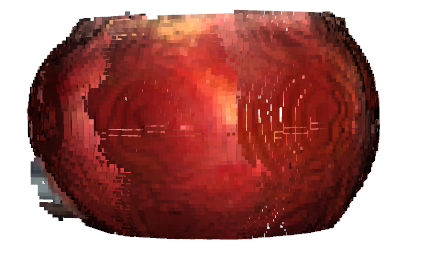
\includegraphics[scale=0.7]{jablko_45_pt.PNG}}
\subcaptionbox{Próbkowanie 11.25\degree}
  [.4\linewidth]{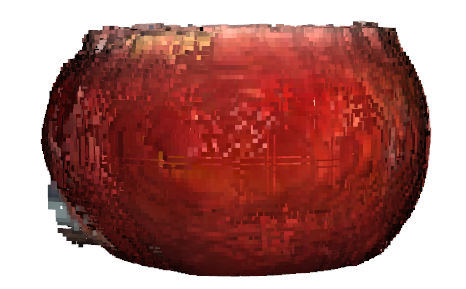
\includegraphics[scale=0.7]{jablko_1125_pt.PNG}}
  \subcaptionbox{Próbkowanie 45\degree}%
  [.4\linewidth]{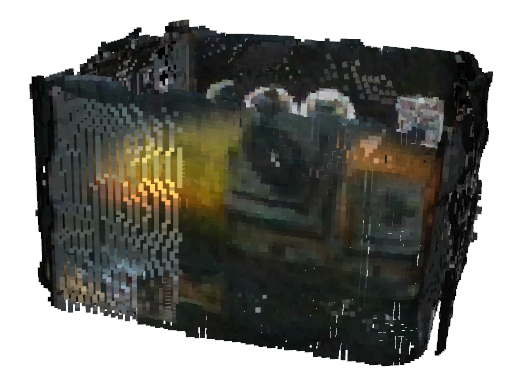
\includegraphics[scale=0.5]{box_global_45_pt.PNG}}
\subcaptionbox{Próbkowanie 11.25\degree}
  [.4\linewidth]{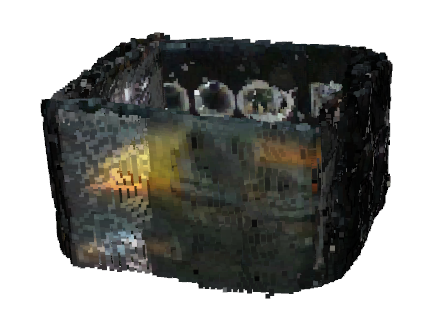
\includegraphics[scale=0.62]{box_global_1125_pt.PNG}}
\caption{Początkowe chmury punktów jabłka oraz pudełka, próbkowane co 45\degree i 11.25\degree}\label{fig:globalInitialCloudsAppleBox}
\end{figure}

Na powyższych rysunkach można zaobserwować, że występują drobne niedoskonałości wynikające z błędnego odczytu danych głębi oraz koloru. Widać to zwłaszcza przy chmurze punktów jabłka. Po boku chmury znajduje się wycinek tła, który powinien mieć większą odległość i zostać usunięty. By tego uniknąć można odfiltrować punkty pod względem koloru. Taki zabieg jednak zmniejszyłby uniwersalność danego rozwiązania.
\newline \indent Ponadto z powyższych chmur wynika obserwacja, że wraz ze wzrostem częstotliwości próbkowania powierzchnia chmury zaczyna być rozmazana. Powodem takiego zachowania są nakładające się na siebie punkty, które są nieznacznie przesunięte względem siebie. Problem ten występuje dla obu chmur i pogłębia się wraz ze wzrostem liczby punktów poddanych obróbce. Dla małej liczby punktów, problem jest niemalże niedostrzegalny. Jednakże, przy próbkowaniu co 11.25$\degree$ ostateczna chmura zawiera ponad 40000 punktów i ten mankament staje się bardziej widoczny.
 \newline \indent Zwiększanie ilości punktów estymacyjnych w metodzie RANSAC wpływa na poprawę wyglądu chmury, jednak rośnie przy tym złożoność obliczeniowa. By osiągnąć najlepsze efekty każdy z parametrów należy dobierać ręcznie w zależności od częstotliwości próbkowania i typu obiektu. Do dalszych analiz wybrano chmurę punktów, dla której próbki wykonywano co 45\degree.

W celu otrzymania siatki triangulacyjnej użyto algorytmu BPA z biblioteki Open3D. Liczba punktów w chmurze wynosiła 27000 oraz 40000, odpowiednio dla jabłka oraz pudełka. Wyniki algorytmu dla długości promienia równych R=3$D_{mean}$ oraz R=5$D_{mean}$, gdzie $D_{mean}$ jest średnią odległością punktów od siebie, zostały przedstawione na rysunku \ref{fig:globalRegisterBpaAppleBox}.
\begin{figure}[H]
\centering
\subcaptionbox{R=3$D_{mean}$}%
  [.4\linewidth]{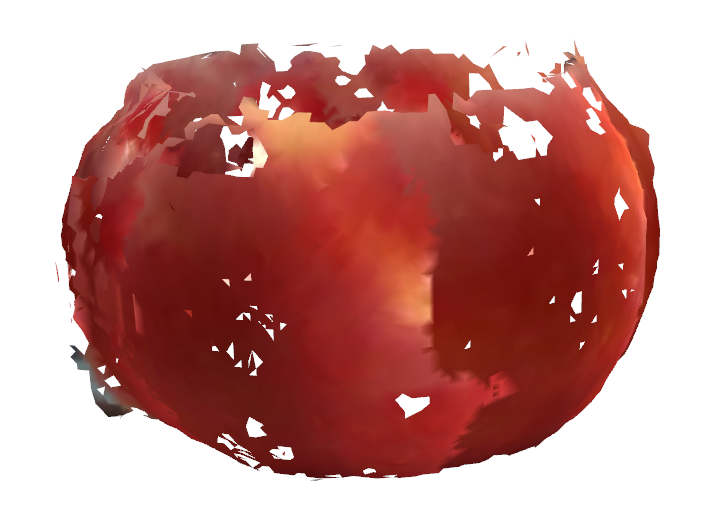
\includegraphics[height=4cm]{bpa_apple_global_45_3dmean.PNG}}
\subcaptionbox{R=5$D_{mean}$}
  [.4\linewidth]{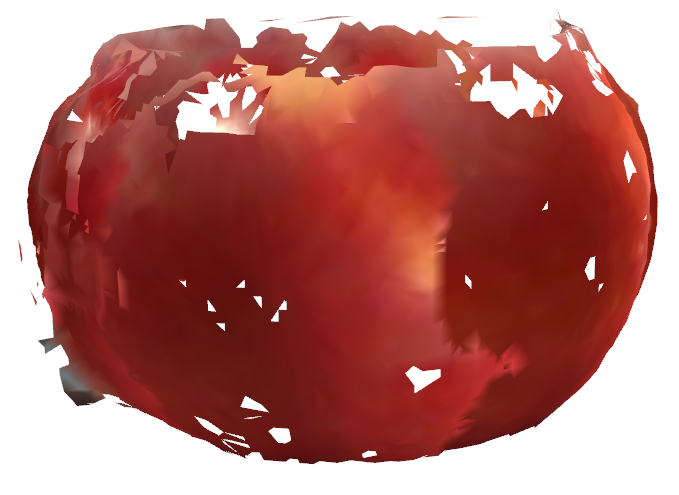
\includegraphics[height=4cm]{bpa_apple_global_45_5dmean.PNG}}
  \subcaptionbox{R=3$D_{mean}$}%
  [.4\linewidth]{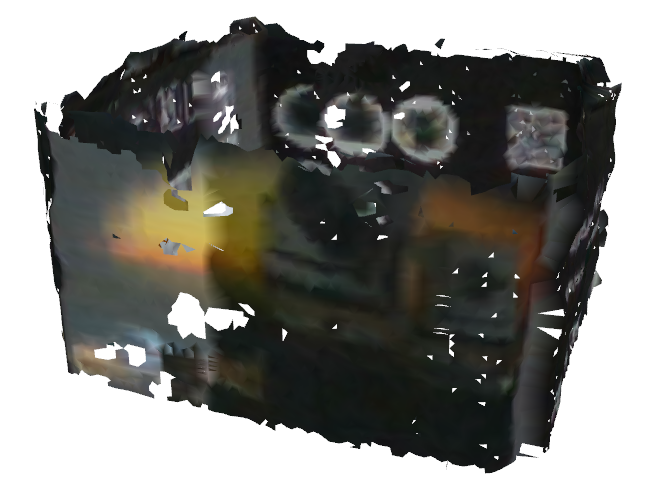
\includegraphics[height=4cm]{bpa_box_global_3dmean.PNG}}
\subcaptionbox{R=5$D_{mean}$}
  [.4\linewidth]{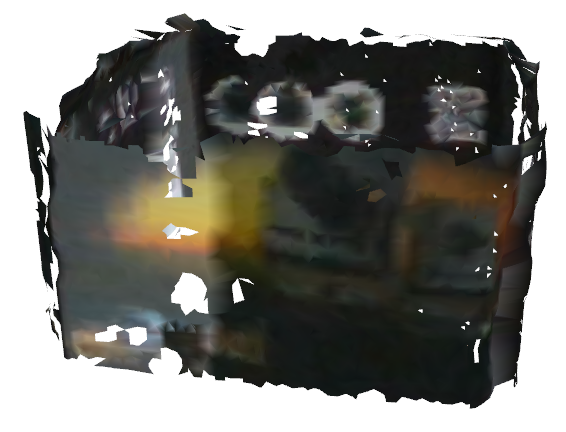
\includegraphics[height=4cm]{bpa_box_global_5dmean.PNG}}
\caption{Siatka utworzona za pomocą algorytmu BPA jabłka oraz pudełka dla promieni R=3$D_{mean}$ oraz R=5$D_{mean}$}\label{fig:globalRegisterBpaAppleBox}
\end{figure} 
Na powyższych rysunkach przedstawiono wpływ długości promienia na ostateczny wygląd siatki wygenerowanej przez algorytm toczącej się kuli. Otrzymane rezultaty nie są jednak zadowalające. Pomimo znacznego zwiększenia liczby oraz gęstości punktów, wyniki znacząco odbiegają od tych otrzymanych przy metodzie skanera liniowego. Ponadto zwiększenie promienia kuli z 3$D_{mean}$ do 5$D_{mean}$ nie zmniejszyło liczby dziur w modelu. Wygląd obiektu zależy w znacznym stopniu od ułożenia punktów. W miejscach, w których się ze sobą pokrywają powstaje gładka powierzchnia. Jednak na łączeniach oraz górze oraz na dole punkty są gorzej dopasowane. Podstawą tego jest działanie algorytmu RANSAC, który ma na celu minimalizację błędu pomiędzy większością punktów. Efekt algorytmu został uzyskany , jednak przez to, iż skrajne punkty nie stanowią większości całego zbioru, zostały one niedokładnie zespolone. W rezultacie powoduje to, że średnia gęstość punktów w chmurze jest znacznie mniejsza niż gęstość punktów na skrajnych powierzchniach. Do wyznaczenia długości promienia kuli można posłużyć się średnią odległością pomiędzy punktami. W przypadku powyższych badań wybrano promień stanowiący trzykrotność oraz pięciokrotność średniej odległości między punktami. Niestety, przez znacznie mniejszą gęstość na krańcach chmury, algorytm nie był w stanie połączyć ze sobą sąsiednich punktów. Skutkowało to występowaniem dziur w obiekcie.
\newline \indent Na rysunku \ref{fig:globalRegisterDelaunayAppleBox} zestawiono wyniki algorytmu triangulacji Delaunay'a utworzone na podstawie jabłka oraz pudełka.
\begin{figure}[H]
\centering
\subcaptionbox{Jabłko}%
  [.4\linewidth]{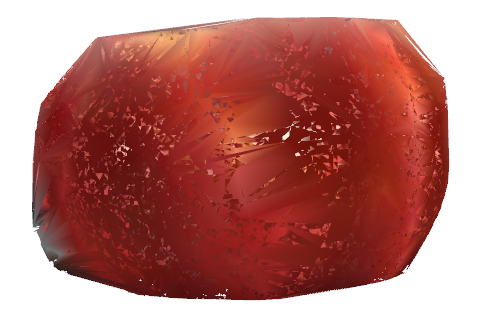
\includegraphics[height=4cm]{delaunay_apple_global_45.PNG}}
\subcaptionbox{Pudełko}
  [.4\linewidth]{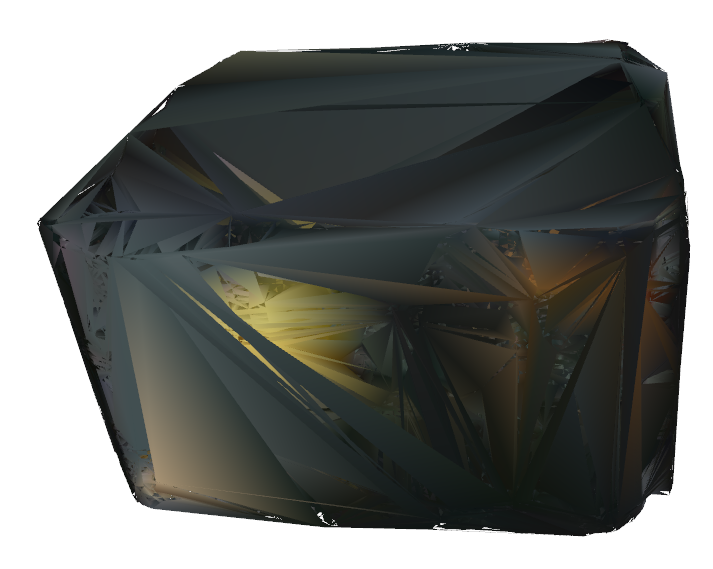
\includegraphics[height=4cm]{delaunay_box_global_45.PNG}} 
\caption{Wyniki triangulacji Delaunay'a}\label{fig:globalRegisterDelaunayAppleBox}
\end{figure}
Na powyższych rysunkach zaprezentowano rezultaty przeprowadzenia triangulacji na dwóch chmurach punktów. Można na nich zaobserwować, że dużo szczegółów powierzchni jest przykrytych. Wynika to z nakładających się ścian utworzonych przez trójkąty triangulacyjne. W dalszej części pracy przedstawiono dokładne omówienie zagadnienia wraz z opracowaniem wyników. Jednakże niewątpliwą zaletą takiego rozwiązania jest brak dziur w powierzchni obiektu. Poprzez zastosowanie takiej metody generacji siatki, można również utworzyć dotychczas nie istniejące ściany. Na rysunkach przedstawione są obiekty, dla których górne ściany nie zostały zeskanowane. Jednak w wyniku przeprowadzenia triangulacji zostały one utworzone. Wykorzystując narzędzia do modelowania oraz obróbki obiektów trójwymiarowych, na przykład Blender, można usunąć część źle rozmieszczonych ścian.
\newline \indent Po przeprowadzeniu analizy wyników można wysnuć wiele wniosków. Na powstałych w rezultacie chmurach punktów dokonano wielu przekształceń, by je ze sobą scalić. Jednakże rezultaty tych działań są niezadowalające. Punkty nie pokrywają się z należytą dokładnością. Ponadto znacznie zwiększyła się liczba punktów w chmurze, nie wpływając przy tym na poprawę wyników. Z kolei znacznie wpłynęło to na zwiększenie złożoności obliczeniowej. Zbiory punktów powstałe w skutek użycia metody skanera liniowego zawierają mniej punktów, generując przy tym lepszy efekt końcowy. Zarówno algorytm BPA jak i triangulacja Delaunay'a dla zastosowanej metody wypadają znacznie gorzej na tle metody skanera liniowego. Po przeprowadzeniu należytych analiz, do dalszego ciągu pracy wybrano metodę skanera liniowego ze względu na jego możliwość dokładniejszego odwzorowania powierzchni obiektu.


